\RequirePackage{amsmath}
\documentclass[runningheads]{llncs}

\usepackage{amssymb}
\usepackage{subfigure}
\usepackage{mathtools}
\usepackage{verbatim}
\usepackage{stmaryrd}
\usepackage{listings}
\usepackage{color}
\usepackage{courier}
\usepackage{xspace}
\usepackage{float}

%\usepackage{amsmath, amssymb, amsfonts}
\usepackage{tikz}
\usetikzlibrary{calc}
\usetikzlibrary{automata}
\usetikzlibrary{positioning,decorations.markings}
\usepackage{filecontents}
\usepackage{listings}
\usepackage{stmaryrd}
\usepackage[margin=1in]{geometry}
%\usepackage{amsthm}

\definecolor{codegreen}{rgb}{0,0.6,0}
\definecolor{codegray}{rgb}{0.5,0.5,0.5}
\definecolor{codepurple}{rgb}{0.58,0,0.82}
\definecolor{backcolour}{rgb}{0.95,0.95,0.92}
\lstdefinestyle{mystyle}{
	stringstyle=\color{codepurple},
	basicstyle=\footnotesize\ttfamily,
	breakatwhitespace=false,         
	breaklines=true,                 
	captionpos=b,                    
	keepspaces=true,                
	numbersep=5pt,                  
	showspaces=false,                
	showstringspaces=false,
	showtabs=false,                  
	tabsize=2
}
\lstset{style=mystyle}

\newcommand{\dom}{\operatorname{dom}}
\newcommand{\im}{\operatorname{im}}
\newcommand{\sem}[1]{\ensuremath{\llbracket #1 \rrbracket}}
\renewcommand{\L}{{\cal L}}
\newcommand{\tc}{T_{\rm c\lca}}
\newcommand{\no}{{\tt null}}
\newcommand{\m}{\underline{m}}
\newcommand{\n}{\underline{n}}
\newcommand{\free}{\operatorname{free}}
\newcommand{\NN}{\mathbb{N}}
\newcommand{\C}{{\cal C}}
\newcommand{\D}{{\cal D}}
\newcommand{\B}{\mathbb{B}}
\newcommand{\F}{\mathbb{F}}
\newcommand{\K}{\mathbb{K}}
\newcommand{\V}{\mathbb{V}}
\newcommand{\W}{\mathbb{W}}

\usetikzlibrary{arrows}
\newcommand{\defn}[1]{Definition~\ref{defn:#1}}
\newcommand{\fig}[2][]{Figure~\ref{fig:#2}\ensuremath{#1}}
\newcommand{\tab}[1]{Table~\ref{tab:#1}}
\newcommand{\eq}[1]{(\ref{eqn:#1})}
\newcommand{\ex}[1]{Example~\ref{ex:#1}}
\newcommand{\secn}[1]{Section~\ref{sec:#1}}
\newcommand{\lem}[1]{Lemma~\ref{lem:#1}}
\newcommand{\cor}[1]{Corollary~\ref{cor:#1}}
\newcommand{\thm}[1]{Theorem~\ref{thm:#1}}
\newcommand{\prop}[1]{Proposition~\ref{prop:#1}}

\newcommand{\ie}{i.e.,\xspace}
\newcommand{\eg}{\emph{e.g.}, \xspace}

%% I changed the symbols to 0,1,+,* to avoid confusion with the meet and join from lattices.
\newcommand{\cbot}{0}
\newcommand{\ctop}{1}
\newcommand{\ctimes}{\times}
\newcommand{\cplus}{+}
\newcommand{\CS}{{\bf CS}}

\pagestyle{plain}

%\long\def\/*#1*/{}

\lstdefinestyle{base}{
	emptylines=1,
	breaklines=false,
	basicstyle=\ttfamily\color{black},
	basicstyle=\footnotesize\ttfamily,
	moredelim=**[is][\color{red}]{@}{@},
}

\begin{document}
\begin{filecontents*}{temp.tikz}
	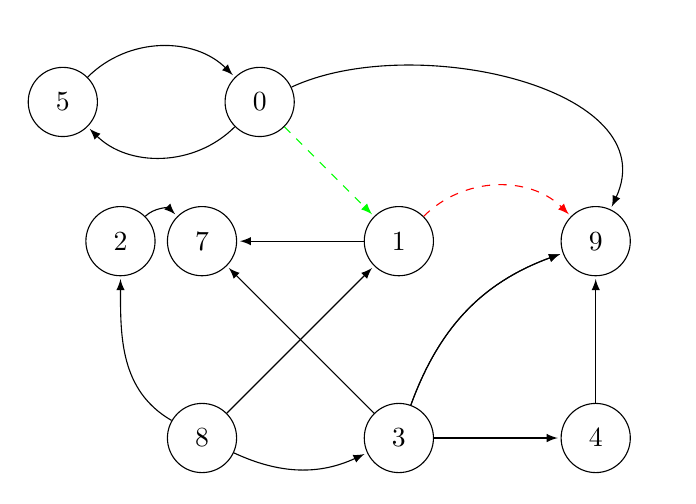
\begin{tikzpicture}[>=latex,shorten >=1pt,node distance=2.5cm,on grid,auto, node/.style={circle,draw=none,minimum size=35pt}, ]
	
	\node[state] (0) at (0pt,0pt) {$0$};
	\node[state, below right = of 0] (1) {$1$};
	\node[state, below left = of 0] (2) {$2$};
	\node[state, below of=1] (3) {$3$};
	\node[state, right = of 3] (4) {$4$};
	\node[state, left = of 0] (5) {$5$};
%	\node[state, right = of 4, fill={rgb:red,1;green,0;blue,0}] (6) {$6$};
	\node[state, below right of= 5] (7) {$7$};
	\node[state, left of= 3] (8) {$8$};
	\node[state, right = of 1] (9) {$9$};

	\draw[->,dashed,draw=green] (0) to[] node[above] {} (1);
	\draw[->] (8) to[] node[above] {} (1);
	\draw[->] (2) to[out=45,in=135] node[right] {} (7);
	\draw[->] (1) to[] node[above] {} (7);
	\draw[->] (3) to[] node[right] {} (4);
	\draw[->] (4) to[] node[above] {} (9);
	\draw[->,dashed,draw=red] (1) to[out=45,in=135] node[right] {} (9);
	\draw[->] (3) to[out=70,in=200] node[above] {} (9);
%	\draw[->,dashed,draw=red] (1) to[out=-45,in=135] node[right] {} (6);	
	\draw[->] (8) to[out=-25,in=205] node[above] {} (3);
	\draw[->] (3) to[out=135,in=-45] node[above] {} (7);
	\draw[->] (8) to[out=150,in=-90] node[right] {} (2);
	\draw[->] (3) to[out=70,in=200] node[above] {} (9);
%	\draw[->,dashed,draw=red] (9) to[out=-20, in=110] node[above] {} (6);
%	\draw[->] (4) to[] node[right] {} (6);	

	\draw[->] (5) to[out=45, in=135] node[above] {} (0);
	\draw[->] (0) to[out=225,in=-45] node[right] {} (5);	
	\draw[->] (0) to[out=25,in=65] node[right] {} (9);
	
	\end{tikzpicture}
\end{filecontents*}
\begin{figure}[H]
	\centering
	\resizebox{5cm}{!}{ 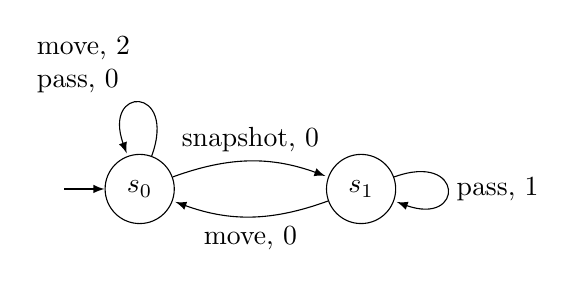
\begin{tikzpicture}[>=latex,shorten >=1pt,node distance=3cm,on grid,auto, node/.style={circle,draw,minimum size=25pt}, ]

 \node[state] (B) at (80pt,0pt) {$s_1$};

 \node[state] (A) at (0pt,0pt) {$s_0$};
 \draw[<-] (A) -- node[above left] {} ++(-1,0);
 \draw[->] (B) to[out=20,in=-20,looseness=8] node[right, align=left] {pass, 1} (B);
 \draw[->] (A) to[out=20,in=160,looseness=1] node[above] {snapshot, 0} (B);
 \draw[->] (B) to[out=200,in=-20,looseness=1] node[below] {move, 0} (A);
 \draw[->] (A) to[out=70,in=110,looseness=8] node[above left, align=left] {move, 2 \\ pass, 0} (A);


 \end{tikzpicture}
}
	\caption{coproduct and universal property}\label{fig:myfigure}
\end{figure}

\begin{filecontents*}{temp.tikz}
	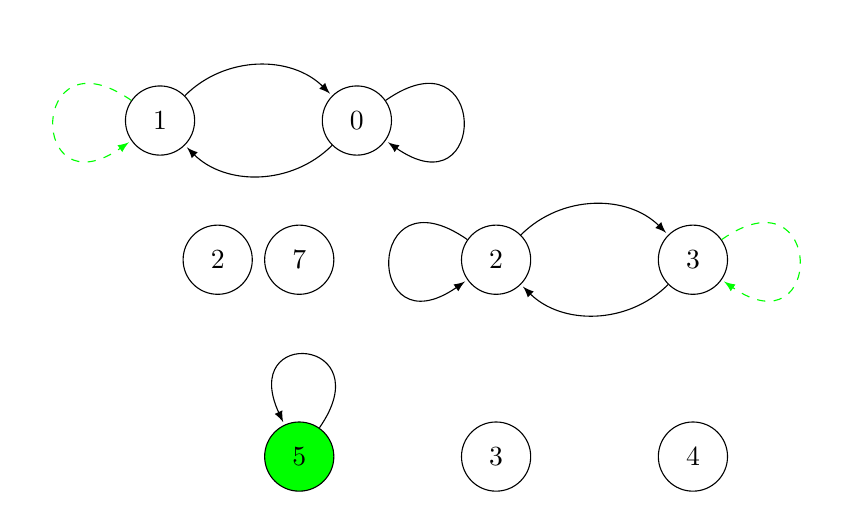
\begin{tikzpicture}[>=latex,shorten >=1pt,node distance=2.5cm,on grid,auto, node/.style={circle,draw=none,minimum size=35pt}, ]
	
	\node[state] (0) at (0pt,0pt) {$0$};
	\node[state, below right = of 0] (1) {$2$};
	\node[state, below left = of 0] (2) {$2$};
	\node[state, below of=1] (3) {$3$};
	\node[state, right = of 3] (4) {$4$};
	\node[state, left = of 0] (5) {$1$};
	\node[state, below right of= 5] (7) {$7$};
	\node[state, left of= 3,fill={rgb:red,0;green,0.5;blue,0}] (8) {$5$};
	\node[state, right = of 1] (9) {$3$};
	

	\draw[->] (1) to[out=45,in=135] node[right] {} (9);
	\draw[->] (9) to[out=225,in=-45] node[right] {} (1);

	\draw[->] (8) to[out=55,in=115,looseness=8] node[above] {} (8);
	\draw[->] (1) to[out=145,in=215,looseness=8] node[above] {} (1);
	\draw[->] (0) to[out=35,in=-35,looseness=8] node[above] {} (0);
	\draw[->,dashed,draw=green] (5) to[out=145,in=215,looseness=8] node[above] {} (5);
	\draw[->,dashed,draw=green] (9) to[out=35,in=-35,looseness=8] node[above] {} (9);
	
	\draw[->] (5) to[out=45, in=135] node[above] {} (0);
	\draw[->] (0) to[out=225,in=-45] node[right] {} (5);	
	
	\end{tikzpicture}
\end{filecontents*}
\begin{figure}[H]
	\centering
	\resizebox{5cm}{!}{ 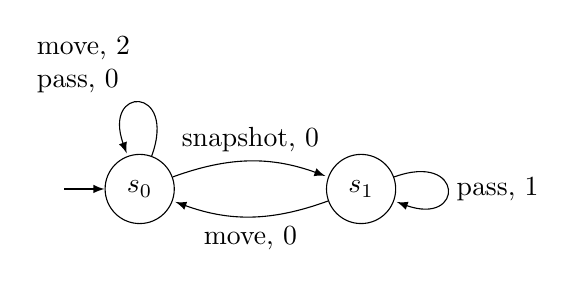
\begin{tikzpicture}[>=latex,shorten >=1pt,node distance=3cm,on grid,auto, node/.style={circle,draw,minimum size=25pt}, ]

 \node[state] (B) at (80pt,0pt) {$s_1$};

 \node[state] (A) at (0pt,0pt) {$s_0$};
 \draw[<-] (A) -- node[above left] {} ++(-1,0);
 \draw[->] (B) to[out=20,in=-20,looseness=8] node[right, align=left] {pass, 1} (B);
 \draw[->] (A) to[out=20,in=160,looseness=1] node[above] {snapshot, 0} (B);
 \draw[->] (B) to[out=200,in=-20,looseness=1] node[below] {move, 0} (A);
 \draw[->] (A) to[out=70,in=110,looseness=8] node[above left, align=left] {move, 2 \\ pass, 0} (A);


 \end{tikzpicture}
}
	\caption{coproduct and universal property}\label{fig:myfigure}
\end{figure}

$$
=
$$

\begin{filecontents*}{temp.tikz}
	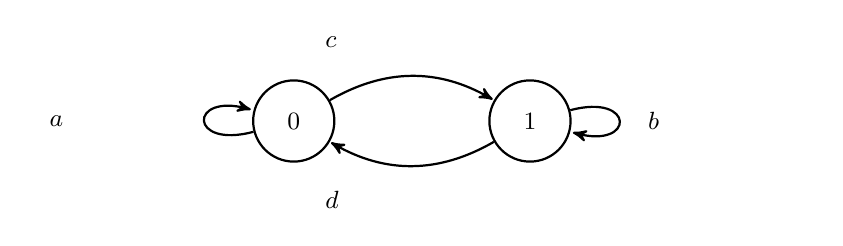
\begin{tikzpicture}[->,>=stealth',shorten >=0.5pt,auto,node distance=3cm,
	thick,main node/.style={circle,draw,font=\sffamily\small}, align=center, text width=2cm]
	
	\node[main node, text width=0.7cm] (1) {$0$};
	\node[main node, text width=0.7cm] (2) [right of=1] {$1$};
	
	\node[align=left,font=\sffamily\small] (A) at (-2.1,0) {$a$};
	\node[align=left,font=\sffamily\small] (B) at (5.5,0) {$b$};
	\node[align=left,font=\sffamily\small] (D) at (1.4,1) {$c$};
	\node[align=left,font=\sffamily\small] (E) at (1.4,-1) {$d$};
	\path[every node/.style={font=\sffamily\small}]
	(1) edge [bend left] node [above,sloped] {} (2)
	edge [loop left] node { } (1)
	(2) edge [bend left] node [below,sloped] {} (1)
	edge [loop right] node { } (2);
	\end{tikzpicture}
\end{filecontents*}
\begin{figure}[htb]
	\centering
	\resizebox{9cm}{!}{ 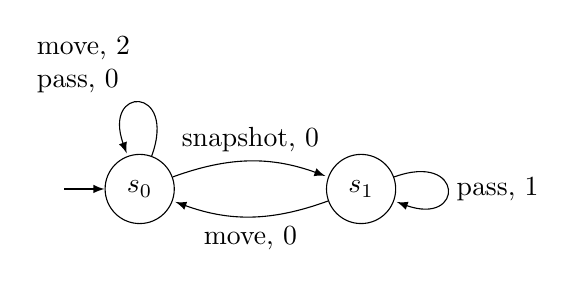
\begin{tikzpicture}[>=latex,shorten >=1pt,node distance=3cm,on grid,auto, node/.style={circle,draw,minimum size=25pt}, ]

 \node[state] (B) at (80pt,0pt) {$s_1$};

 \node[state] (A) at (0pt,0pt) {$s_0$};
 \draw[<-] (A) -- node[above left] {} ++(-1,0);
 \draw[->] (B) to[out=20,in=-20,looseness=8] node[right, align=left] {pass, 1} (B);
 \draw[->] (A) to[out=20,in=160,looseness=1] node[above] {snapshot, 0} (B);
 \draw[->] (B) to[out=200,in=-20,looseness=1] node[below] {move, 0} (A);
 \draw[->] (A) to[out=70,in=110,looseness=8] node[above left, align=left] {move, 2 \\ pass, 0} (A);


 \end{tikzpicture}
}
	\caption{East-West soft constraint automaton}\label{fig:myfigure}
\end{figure}

\begin{filecontents*}{temp.tikz}
	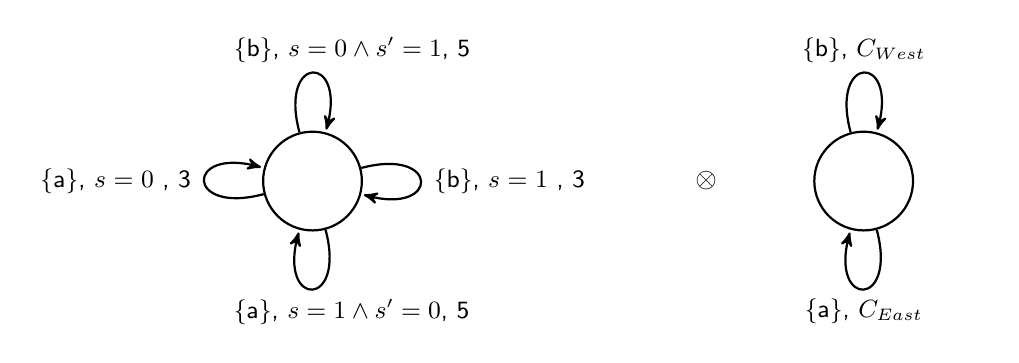
\begin{tikzpicture}[->,>=stealth',shorten >=0.5pt,auto,node distance=3cm,
	thick,main node/.style={circle,draw,font=\sffamily\small}, align=center, text width=2cm]
	
	\node[main node, text width=1cm] (1) at (-2,0) {};
	\node at (3,0) {$\otimes$};
	\node[main node, text width=1cm] (2) at (5,0) {};
	
	\node[align=left,font=\sffamily] (A) at (-2.1,0) {};
	\node[align=left,font=\sffamily\small] (B) at (5.5,0) {};
	\node[align=left,font=\sffamily\small] (D) at (1.4,1) {};
	\node[align=left,font=\sffamily\small] (E) at (1.4,-1) {};
	\path[every node/.style={font=\sffamily\small}]
	(1) edge [loop above] node [above,align=left] {\text{\{b\}, $s=0 \land s'=1$, 5}} (1)
	edge [loop left] node {\{a\}, $s=0$ , 3} (1)
	(1) edge [loop below] node [below,sloped] {\text{\{a\}, $s=1 \land s'=0$, 5}} (1)
	edge [loop right] node {\{b\}, $s=1$ , 3} (1)
	
	(2) edge [loop above] node [above,sloped] {\{b\}, $C_{West}$} (2)
	edge [loop below] node [below, sloped] {\{a\}, $C_{East}$} (2);
	
	
	\end{tikzpicture}
\end{filecontents*}
\begin{figure}[htb]
	\centering
	\resizebox{12cm}{!}{ 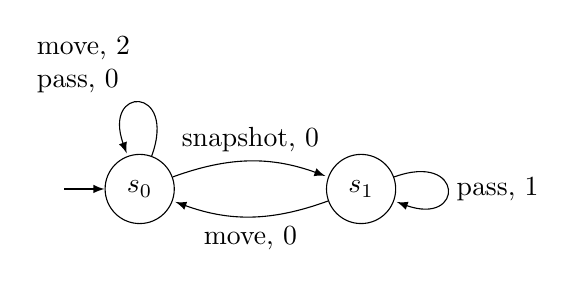
\begin{tikzpicture}[>=latex,shorten >=1pt,node distance=3cm,on grid,auto, node/.style={circle,draw,minimum size=25pt}, ]

 \node[state] (B) at (80pt,0pt) {$s_1$};

 \node[state] (A) at (0pt,0pt) {$s_0$};
 \draw[<-] (A) -- node[above left] {} ++(-1,0);
 \draw[->] (B) to[out=20,in=-20,looseness=8] node[right, align=left] {pass, 1} (B);
 \draw[->] (A) to[out=20,in=160,looseness=1] node[above] {snapshot, 0} (B);
 \draw[->] (B) to[out=200,in=-20,looseness=1] node[below] {move, 0} (A);
 \draw[->] (A) to[out=70,in=110,looseness=8] node[above left, align=left] {move, 2 \\ pass, 0} (A);


 \end{tikzpicture}
}
	\caption{Single state East-West soft constraint automaton}\label{fig:myfigure}
\end{figure}

\begin{filecontents*}{temp.tikz}
	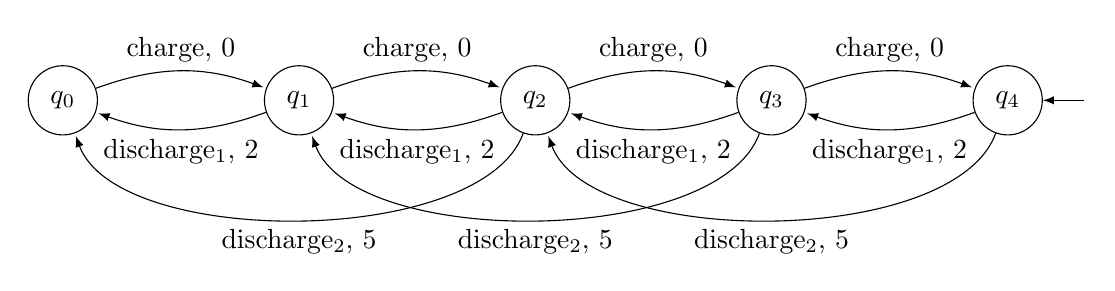
\begin{tikzpicture}[>=latex,shorten >=1pt,node distance=3cm,on grid,auto, node/.style={circle,draw,minimum size=25pt}, ]
	
	\node[state] (q0) at (-40pt,0pt) {$q_0$};
	\node[state, right = of q0] (q1) {$q_1$};
	\node[state, right = of q1] (q2) {$q_2$};
	\node[state, right = of q2] (q3) {$q_3$};
	\node[state, right = of q3] (q4) {$q_4$};
	\draw[<-] (q4) -- node[above right] {} ++(1,0);
	\draw[->] (q1) to[out=200,in=-20] node[below] {discharge$_1$, 2} (q0);
	\draw[->] (q0) to[out=20,in=160] node[above] {charge, 0} (q1);
	\draw[->] (q2) to[out=-110,in=-70,looseness=0.7] node[below] {discharge$_2$, 5} (q0);
	\draw[->] (q2) to[out=200,in=-20] node[below] {discharge$_1$, 2} (q1);
	\draw[->] (q1) to[out=20,in=160] node[above] {charge, 0} (q2);
	\draw[->] (q3) to[out=-110,in=-70,looseness=0.7] node[below] {discharge$_2$, 5} (q1);
	\draw[->] (q3) to[out=200,in=-20] node[below] {discharge$_1$, 2} (q2);
	\draw[->] (q2) to[out=20,in=160] node[above] {charge, 0} (q3);
	\draw[->] (q4) to[out=-110,in=-70,looseness=0.7] node[below] {discharge$_2$, 5} (q2);
	\draw[->] (q4) to[out=200,in=-20] node[below] {discharge$_1$, 2} (q3);
	\draw[->] (q3) to[out=20,in=160] node[above] {charge, 0} (q4);
	\end{tikzpicture}
\end{filecontents*}
\begin{figure}[htb]
	\centering
	\resizebox{16cm}{!}{ 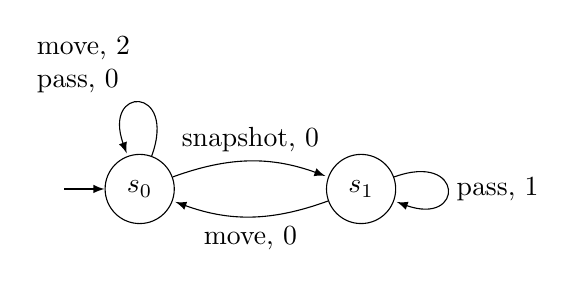
\begin{tikzpicture}[>=latex,shorten >=1pt,node distance=3cm,on grid,auto, node/.style={circle,draw,minimum size=25pt}, ]

 \node[state] (B) at (80pt,0pt) {$s_1$};

 \node[state] (A) at (0pt,0pt) {$s_0$};
 \draw[<-] (A) -- node[above left] {} ++(-1,0);
 \draw[->] (B) to[out=20,in=-20,looseness=8] node[right, align=left] {pass, 1} (B);
 \draw[->] (A) to[out=20,in=160,looseness=1] node[above] {snapshot, 0} (B);
 \draw[->] (B) to[out=200,in=-20,looseness=1] node[below] {move, 0} (A);
 \draw[->] (A) to[out=70,in=110,looseness=8] node[above left, align=left] {move, 2 \\ pass, 0} (A);


 \end{tikzpicture}
}
	\caption{Soft constraint automata for energy management}\label{fig:myfigure}
\end{figure}


\end{document}


